\section{Principio de funcionamiento} 
Si bien en el diseño no se tiene un transformador ideal, es importante entender el principio de funcionamiento de un transformador ideal, ya que este nos permite acercarnos a el funcionamiento del transformador real y de allí pasar al diseño del tramsformador.

\subsection{Transformador ideal}

\begin{figure}[ht!]
    \centering
    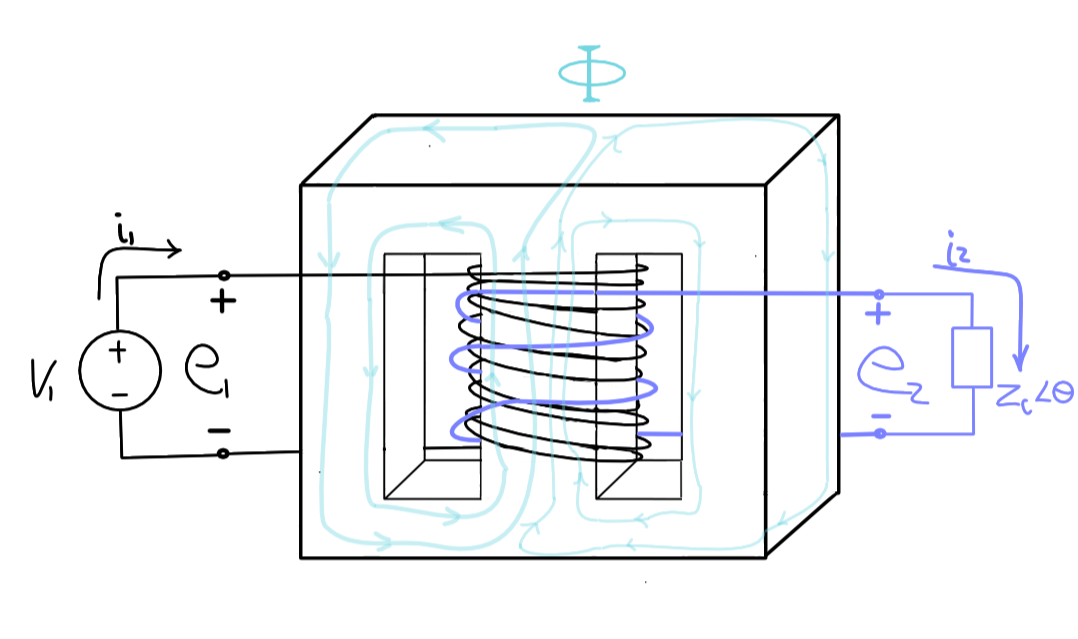
\includegraphics[width=0.48\textwidth]{fot/T4.png}
    \caption{Modelo de tramsformador ideal.}
    \label{fig:T4}
\end{figure}

A partir de la ley de Faraday-Lenz, se establece que la fuerza electromotriz (fem) inducida en un circuito es proporcional a la rapidez de cambio del flujo magnético a través de él. Resultado para una bobina La ecuación que describe esta relación es la siguiente:
\begin{equation}
    \label{eqn1}
    e_1 = N_1 \cdot \frac{d\Phi}{dt}
\end{equation}


\addcontentsline{toc}{section}{Nomenclature}
\begin{IEEEdescription}[\IEEEsetlabelwidth{$V_1,V_2,$}]
\item[e] F.e.m inducida en la bobina.
\mbox{}
\item[$N$] Número de vueltas de la bobina.
\item[$\Phi$] Flujo magnético a través de la bobina.
\end{IEEEdescription}

\vspace{0.5cm}
Si se tiene que la fuente es una sinusoide, el flujo magnético es:
\begin{equation}
    \Phi = \Phi_m \cdot \sin(\omega t)
\end{equation}

Puesto que es un transformador ideal, la f.e.m. inducida en el primario es igual a la tensión de entrada, por lo que se puede escribir la ecuación \ref{eqn1} como:

\begin{center}
    $V_1 = N_1 \cdot \frac{d\Phi}{dt} = N_1 \cdot \frac{d}{dt}(\Phi_m \cdot \sin(\omega t))$
    \\
    $= N_1 \cdot \Phi_m \cdot \omega \cdot \cos(\omega t) [V]$
    \\
    $V_1 = \frac{N_1 \cdot \Phi_m \cdot \omega}{\sqrt{2}}\cdot  [Vrms]$
\end{center}
\begin{equation}
    \label{eqn2}
    V_1 =N_1 \cdot \Phi_m \cdot \frac{f \cdot 2\pi}{\sqrt{2}} [Vrms]
\end{equation}
\vspace{0.3cm}

Tenemos la ley de Gauss para campo magnético, que establece que el flujo magnético a través de una superficie cerrada es igual a la integral de la densidad de flujo magnético a través de esa superficie. La ecuación que describe esta relación es la siguiente:
\begin{equation}
    \label{eqn3}
    \Phi = \int_S \mathbf{B} \cdot d\mathbf{S}
\end{equation}
Como la sección transversal del núcleo es cuadrada, se puede escribir la ecuación \ref{eqn3} como: $\Phi = B \cdot S$
\\
Finalmente de la ecuación \ref{eqn3} en \ref{eqn2} despejando para N se obtiene:
\\
\begin{equation}
    \label{eqn4}
    N_1 = \frac{V_{1rms}}{\Phi_m \cdot f \cdot \frac{2\pi}{\sqrt{2}}} = \frac{V_{1rms}}{B\cdot S\cdot f \cdot \frac{2\pi}{\sqrt{2}}} [vueltas] 
\end{equation}
\\
\addcontentsline{toc}{section}{Nomenclature}
\begin{IEEEdescription}[\IEEEsetlabelwidth{$e,N,S$}]
\item[$f$] frecuencia de la fuente.
\mbox{}
\item[$V_{1rms}$] Tensión eficaz en el primario.
\item[$\Phi$] Flujo magnético a través del arrollamiento.
\item[$B$] densidad de flujo magnético.
\item[$S$] Sección transversal del núcleo. 
\end{IEEEdescription}
\vspace{1cm}


\begin{IEEEeqnarraybox*}{rCl}
    \text{Transformador ideal:} & \text{Transformador real:} \\
    \text{Sin pérdidas} & \text{Con pérdidas} \\
    \text{Sin resistencia} & \text{Con resistencia} \\
    \text{Sin reactancia} & \text{Con reactancia} \\
    \text{Sin saturación} & \text{Con saturación} \\
    \text{Sin fuga de flujo} & \text{Con fuga de flujo}
\end{IEEEeqnarraybox*}